\section{Interface com Utilizador}

A escolha de face efectua-se desenhando exclusivamente sobre a face.
A escolha de aresta efectua-se cruzando a mesma, tendo in�cio numa das suas faces vizinhas e acabando na outra.
A figura \ref{fig:selection} ilustra este processo.


\begin{figure}[ht]
	\centering
	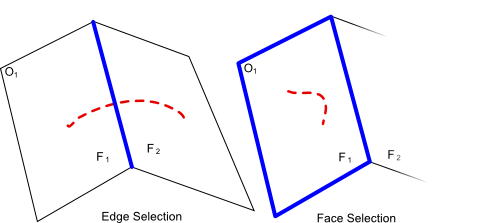
\includegraphics[width=0.8\linewidth]{face-edge-selection.png}
	\vspace{-3mm}
	\caption{selec��o de aresta e de face}
	\label{fig:selection}
	\vspace{-3mm}
\end{figure}

Uma vez escolhido o componente, um menu contextual surge, permitindo a escolha
de uma opera��o a aplicar (ver figura \ref{fig:contextual}).

\begin{figure}[!h]
	\centering
	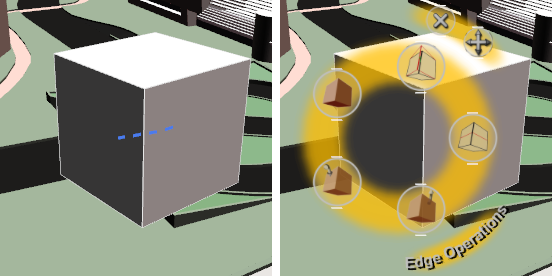
\includegraphics[width=0.65\linewidth]{contextual.png}
	\vspace{-3mm}
	\caption{activa��o de menu contextual de aresta}
	\label{fig:contextual}
	\vspace{-3mm}
\end{figure}

Em diversas opera��es suportadas um dos par�metros � a direc��o.
Quando assim �, entra em funcionamento o algoritmo de escolha de direc��o .
A direc��o do tra�o efectuado � comparada com os diversos sugeridos, aplicando-se
a que mais se aproximar do mesmo, mecanismo popularizado como \textit{snapping}.
% (ver figura \ref{fig:election}).
%Este mecanismo � denominado no software da especialidade como \textit{snapping}.
%
%\begin{figure}[!h]
%	\centering
%	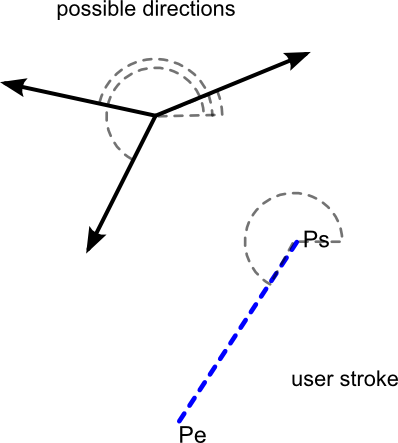
\includegraphics[width=0.35\linewidth]{election.png}
%	\caption{elei��o do vector mais pr�ximo}
%	\label{fig:election}
%\end{figure}

%A figura \ref{fig:icons} lista as opera��es suportadas e respectivos �cones.
%
%\begin{figure}[ht]
%	\centering
%	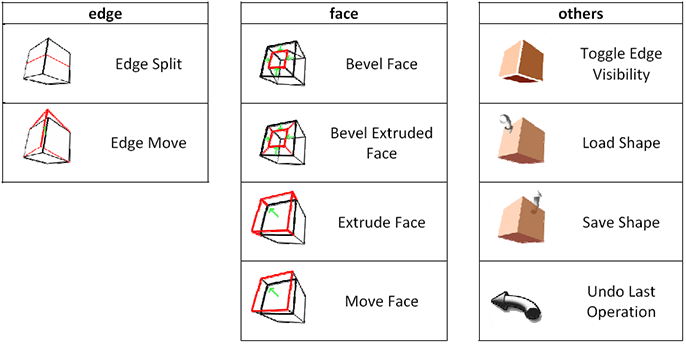
\includegraphics[width=0.94\linewidth]{icons.png}
%	\label{fig:icons}
%	\caption{opera��es dispon�veis por menu e respectivos �cones}
%\end{figure}
